\section{Butcher}

\begin{frame}[plain]{}
    \sectionpage
\end{frame}

\begin{frame}{Introduction}
    Now that the model is successfully imported, the next phase consists of tying to find the "optimal" partitions of the NN. To be able to do this, we will employ the K shortest path method onto a modified version of the original graph.
    
    The main steps that will be performed are:
    \begin{enumerate}
        \item Construction of the "block" graph, a reduced version of the original graph that takes into account the different devices
        \item Removal of the unfeasible paths (due to the memory constraint)
        \item Generation of the final weights
    \end{enumerate}
    
    After this steps, the K shortest path method will be performed onto the new graph
\end{frame}

\begin{frame}[allowframebreaks]{Block graph}
    To simplify the problem, we decided that no more than a link is allowed between the different partitions. This means that some theoretically possible partitions are not considered. 
    
    For this reason, we construct a second graph of type WGraph$<$std::set$<$node\_id\_type$>>$. Every node of this graph contains at least a node of the original graph. We insert in the same node of the new graph all the nodes of the original graph between which a partition cannot be formed.
    
        \begin{figure}[h]
        \centering
    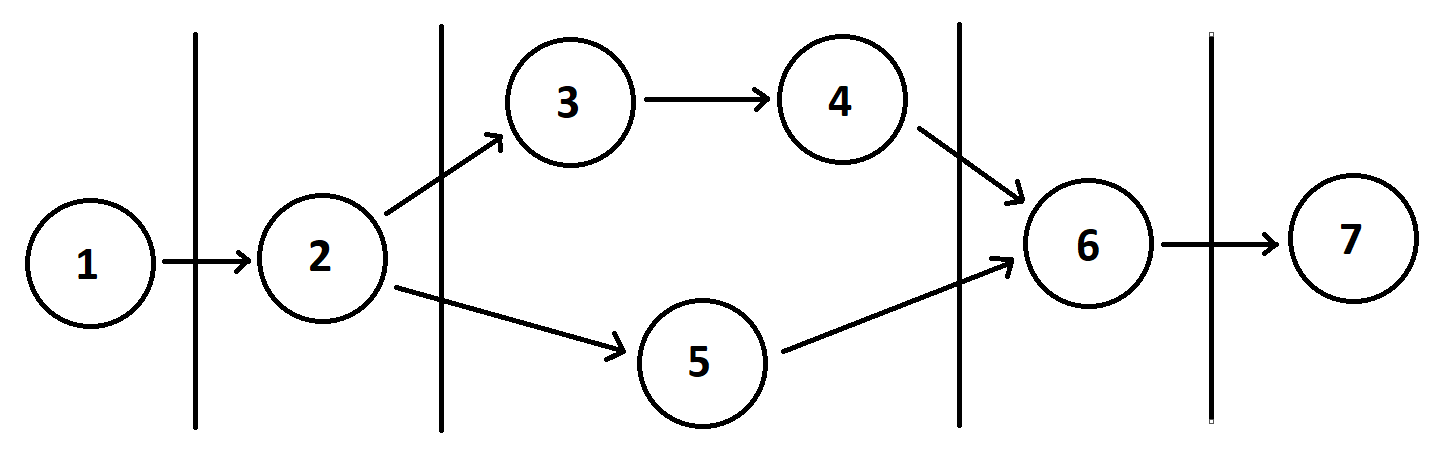
\includegraphics[width=0.4\linewidth]{Img/butcher/basic_graph.png}
    \caption{A graph. The vertical lines represent the different possible ways of partitioning the graph}
    \end{figure}
    
    \framebreak
    
    After this graph is constructed, extra nodes are added based on the number of devices: every node in the new graph should represent a specific collection of nodes in the original graph and a specific device. In this way, during the execution of the K shortest path algorithm, a path in the new graph will represent different partition elements of the network and the devices onto which they should be executed.
    
    \framebreak
    
        \begin{figure}[h]
        \centering
    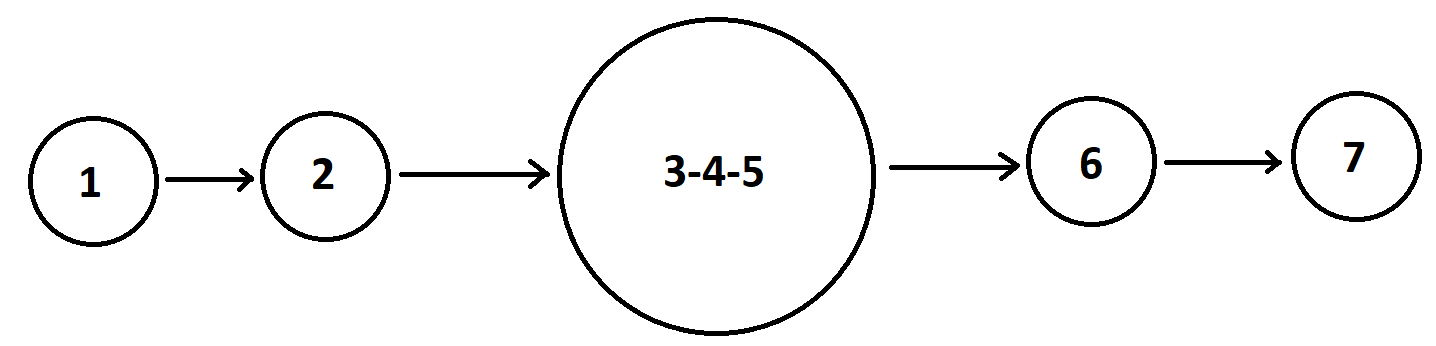
\includegraphics[width=0.4\linewidth]{Img/butcher/linearized_graph.png}
    \caption{First step in block graph construction}
    \end{figure}
    
    \begin{multicols}{2}
        \begin{figure}[h]
        \centering
    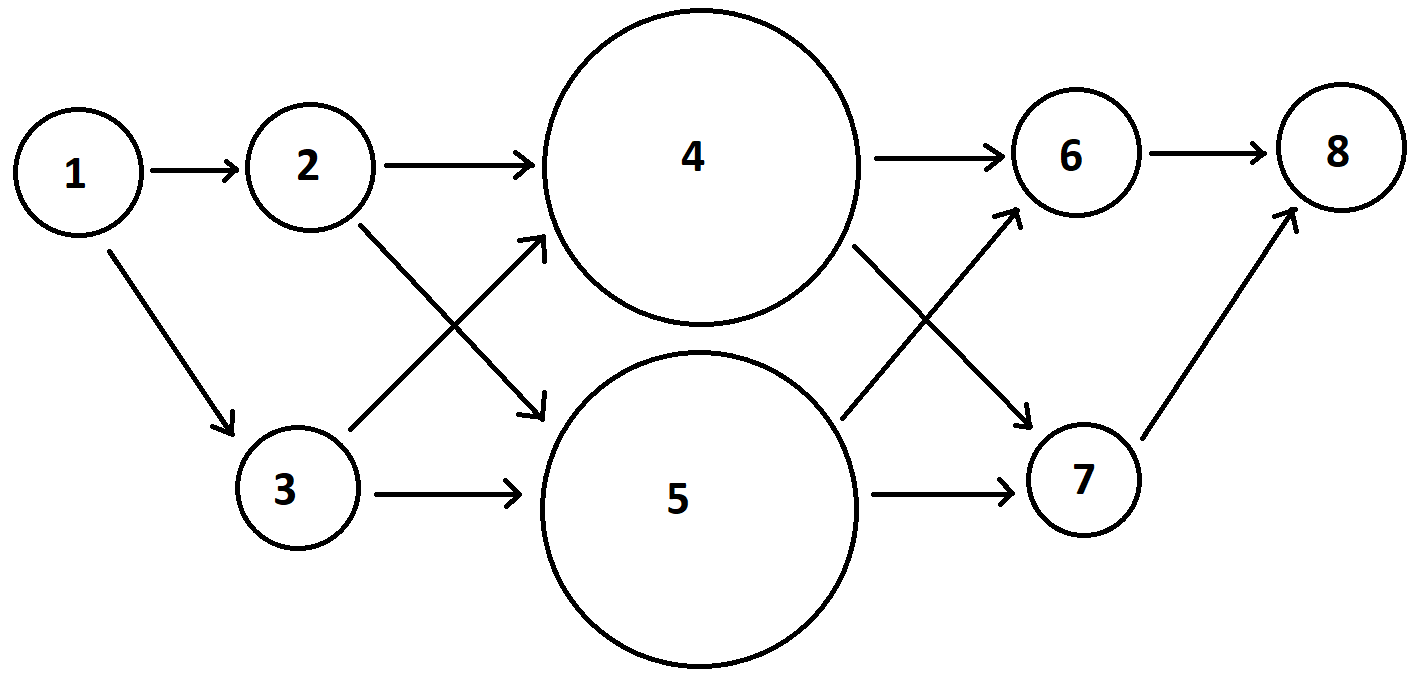
\includegraphics[width=0.75\linewidth]{Img/butcher/block_graph.png}
    \caption{The block graph}
    \end{figure}
    
        \begin{figure}[h]
        \centering
    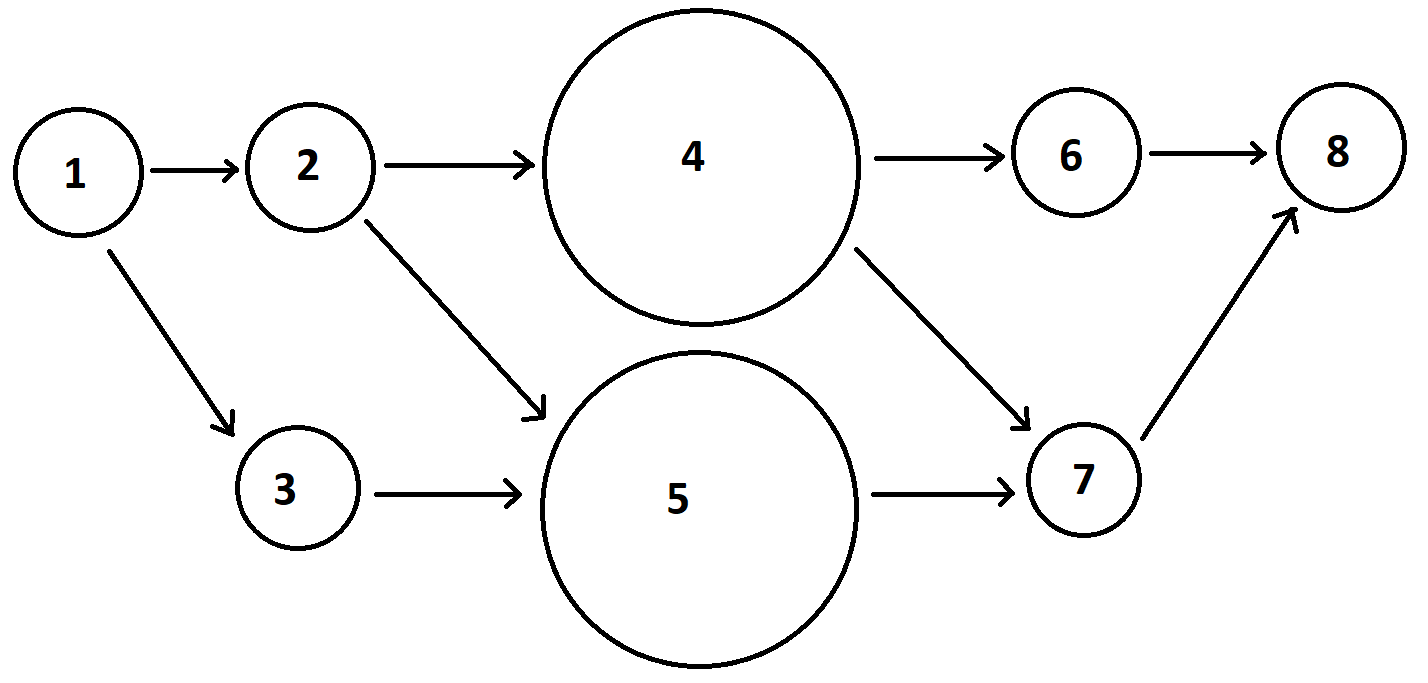
\includegraphics[width=0.75\linewidth]{Img/butcher/block_graph_no_backward_connections.png}
    \caption{The block graph (no backward connections)}
    \end{figure}
    \end{multicols}
    
    
    
\end{frame}

\begin{frame}{Memory constraint}
    \begin{block}{Basic idea}
    Every device has a maximum allowed memory capacity allocated for the execution of the NN. This means that, in theory, a partition of a NN may not be executable on a specific device. For this reason, based on the specified memory\_constraint\_type, some nodes and links in the block graph can be "safely" removed, since they are associated to unfeasible partitions.
    \end{block}
    
    If a node in the block graph corresponds to a single node in the original graph, we just measure the memory required by the input and output tensors. 
    
    If the node corresponds to multiple node in the original graph, we estimate the maximum memory required overall by this "block". 
    
    This estimate is done by computing the maximum input and output tensor dimensions and multiplying their sum by the number of tensors that, in the worst case, must be stored in memory.
\end{frame}

\begin{frame}{Import weights}
    The weights can be imported into the MWGraph through .csv files. There are three available import options:
    \begin{itemize}
        \item aMLLibrary: the .csv file is in the same format as the output file of the testing phase of the python aMLLibrary library. Note that, with this mode, only the weights associated to the convulutional layers are imported. 
        \item operation\_time: the .csv file is structured in a simple way: OperationTypeName,Weight. In this case, the program will read the operation reported in the .csv file and it will loop thorugh the nodes of the graph until the associated node is found. It will then add the related weight to the specified device
        \item multi\_operation\_time: the .csv file is structured in a simple way: OperationTypeName,Weight0,Weight1,... . In this case, the program will read the operation reported in the .csv file and it will loop through the nodes of the graph until the associated node is found. It will then add the related weights to all the devices
    \end{itemize}
\end{frame}

\begin{frame}{Transmission function}
    Since the objective of the program is to compute the optimal partitions for a given NN to be executed on different devices, we have to take into account that sending data from a device to another has a cost. 
    
    This cost is related to the memory space of the tensor to be sent. Moreover, this depends on the type of connection between the devices. 
    
    To simplify this process, we consider a transmission function that, based on the bandwidth parameters and the dimension of the tensor to be transmitted, will produce the related weight.
\end{frame}

\begin{frame}[allowframebreaks]{Weight generation}

    By "construction", the weight of a link represents the time required to transmit the tensor to another device (if needed) and the time required to execute the "input" node on the device specified by the "output" node.
    
    In the block graph, the weight of a link between two nodes is computed in the following way:
    \begin{itemize}
        \item If both nodes are associated to a single node in the original graph, then the resulting weight is given by the transmission cost and the weight between the corresponding nodes in the original graph on the device of the second node
        
    \begin{multicols}{2}
        \begin{figure}[h]
        \centering
    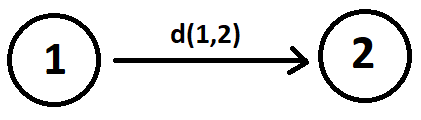
\includegraphics[width=0.5\linewidth]{Img/butcher/simple_edge.PNG}
    \caption{Edge in the original graph}
    \end{figure}
    
        \begin{figure}[h]
        \centering
    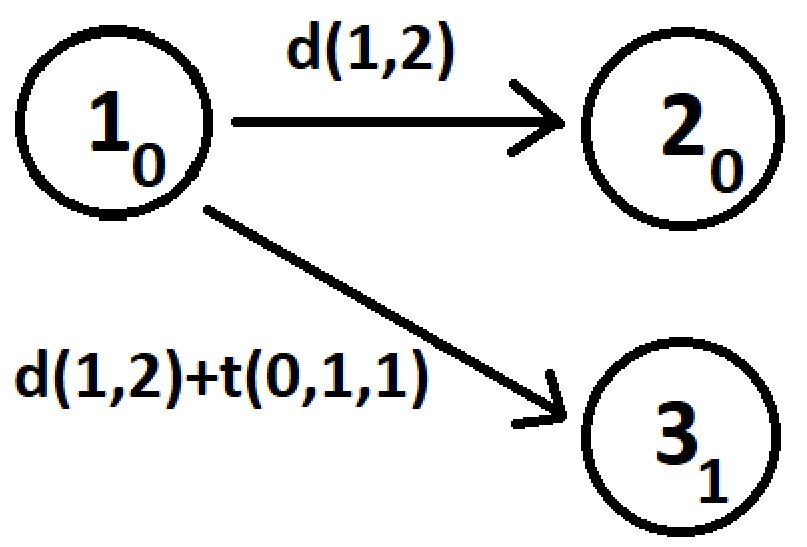
\includegraphics[width=0.4\linewidth]{Img/butcher/block_edge.PNG}
    \caption{Related edges in the block graph}
    \end{figure}
    \end{multicols}
        
        \framebreak
        
        \item If the first node corresponds to a single node in the original graph while the second one to multiple nodes, then the transmission cost for the output tensor of the first node is summed with the different weights between the first node correspondent on the original graph with the "children" nodes in the original graph, plus all the costs between the nodes contained in the second node of the new graph
        
        
    \begin{multicols}{2}
        \begin{figure}[h]
        \centering
    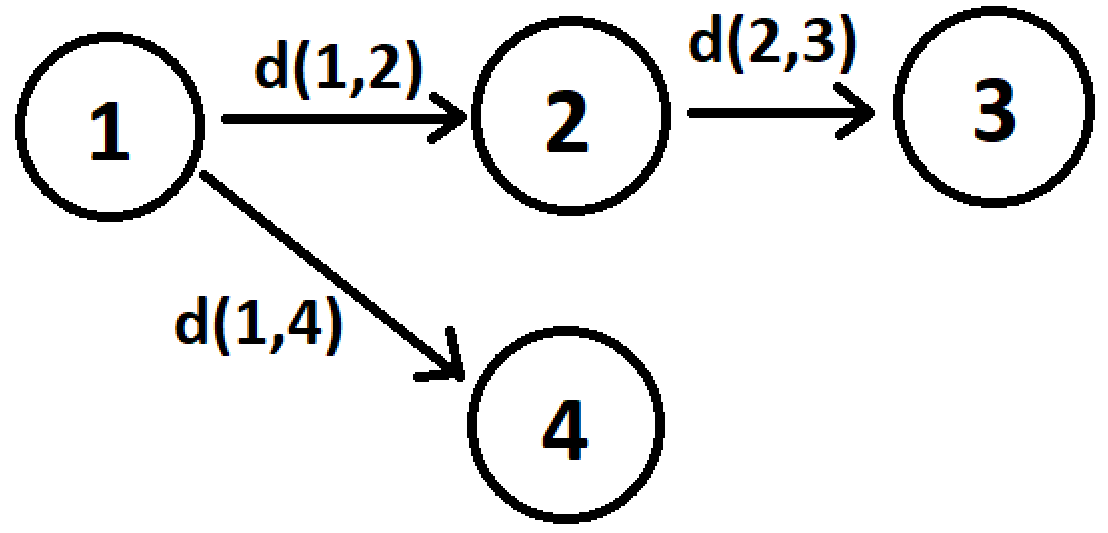
\includegraphics[width=0.5\linewidth]{Img/butcher/2_1_simple_edge.PNG}
    \caption{Edge in the original graph}
    \end{figure}
    
        \begin{figure}[h]
        \centering
    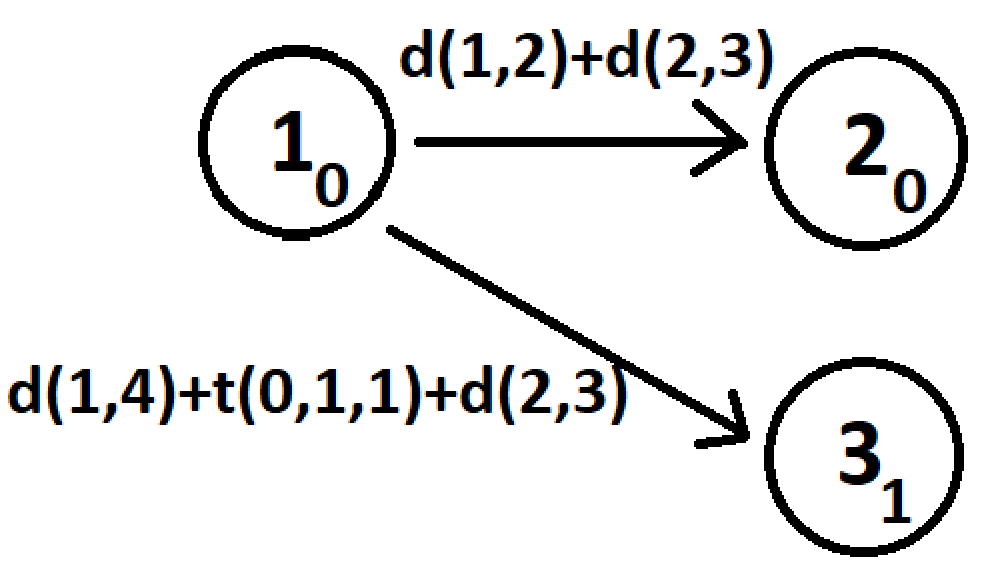
\includegraphics[width=0.7\linewidth]{Img/butcher/2_1_block_edge.PNG}
    \caption{Related edges in the block graph}
    \end{figure}
    \end{multicols}
        
        \framebreak
        
        \item If the first node corresponds to multiple nodes in the original graph while the second one to a single node, then the transmission cost is considered for all the tensors that must be transmitted to the second node plus the costs associated to the links between the input nodes (on the original graph) of the second node in the new graph
        
        
    \begin{multicols}{2}
        \begin{figure}[h]
        \centering
    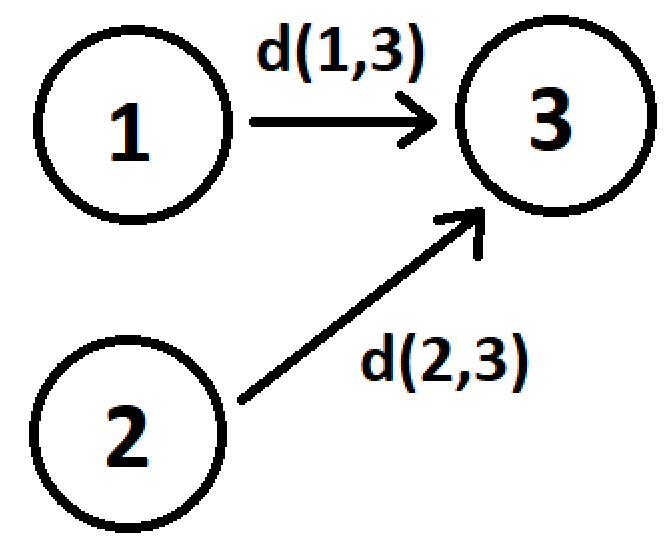
\includegraphics[width=0.4\linewidth]{Img/butcher/1_2_simple_edge.PNG}
    \caption{Edge in the original graph}
    \end{figure}
    
        \begin{figure}[h]
        \centering
    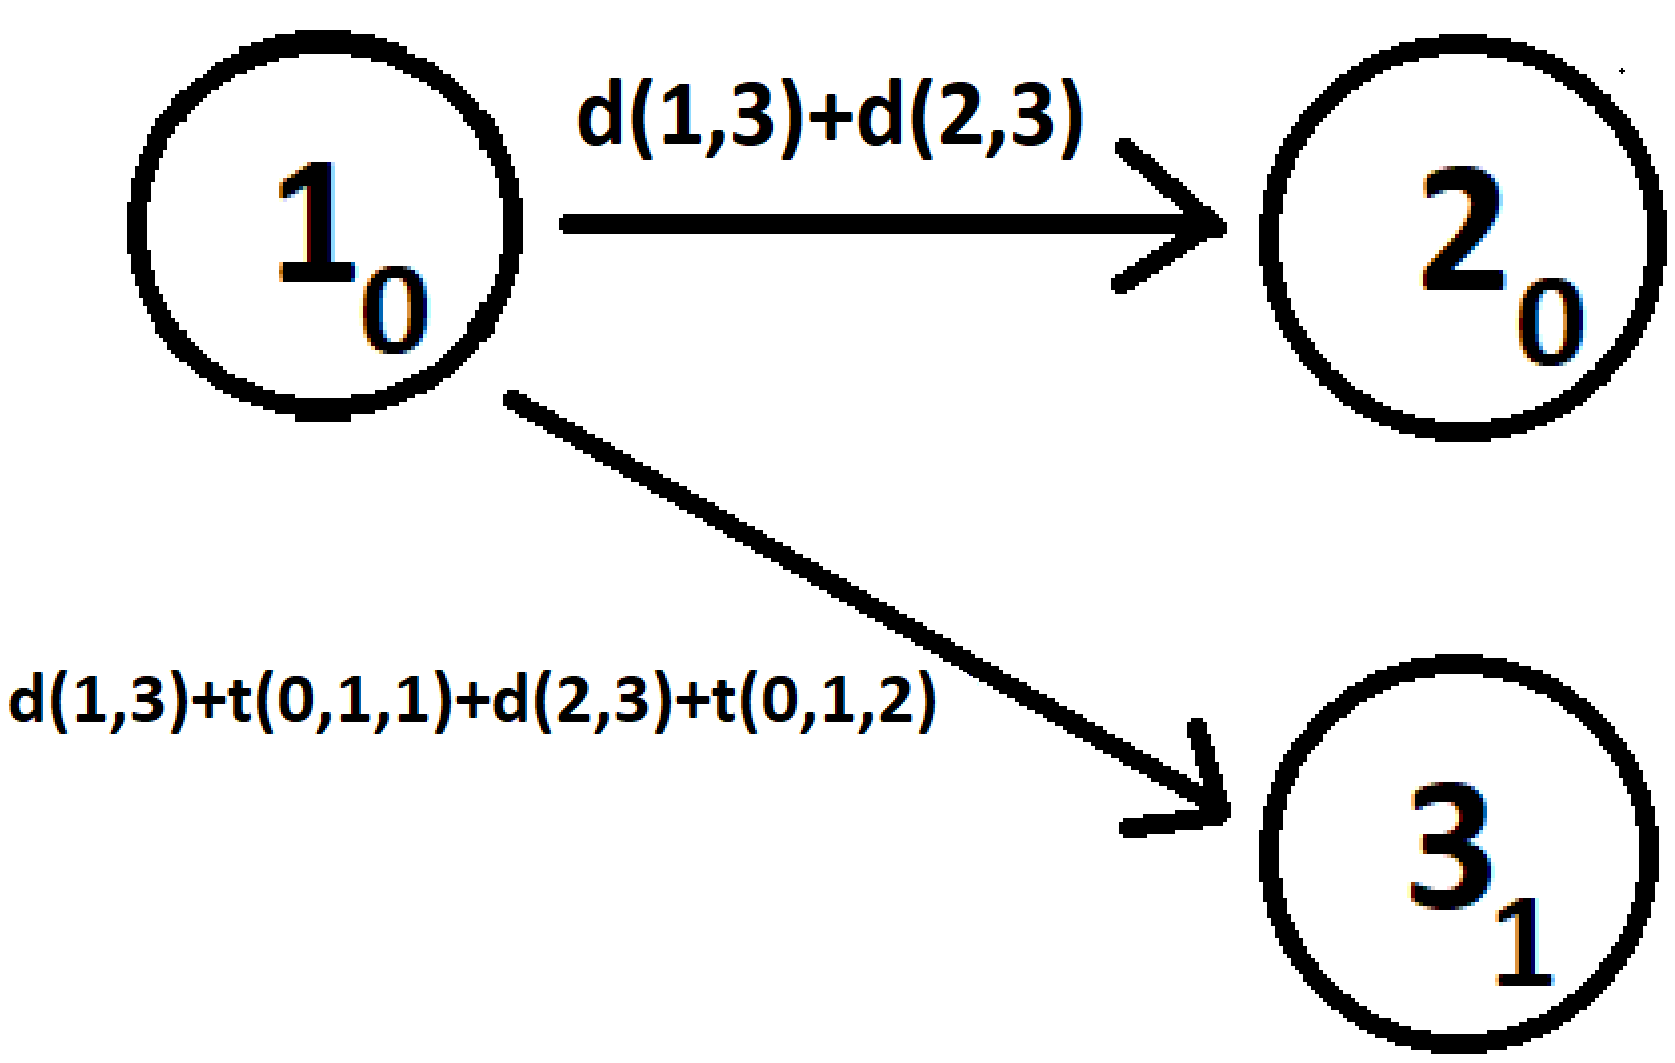
\includegraphics[width=0.6\linewidth]{Img/butcher/1_2_block_edge.PNG}
    \caption{Related edges in the block graph}
    \end{figure}
    \end{multicols}
    
    \end{itemize}
    
\end{frame}